% CVPR 2027 Paper Template; see https://github.com/cvpr-org/author-kit

\documentclass[10pt,twocolumn,letterpaper]{article}

%%%%%%%%% PAPER TYPE  - PLEASE UPDATE FOR FINAL VERSION
% \usepackage{cvpr}              % To produce the CAMERA-READY version
\usepackage[review]{cvpr}      % To produce the REVIEW version
% \usepackage[pagenumbers]{cvpr} % To force page numbers, e.g. for an arXiv version

% Import additional packages in the preamble file, before hyperref
%% This file contains a number of tweaks that are typically applied to the main document.
%% They are not enabled by default, but can be enabled by uncommenting the relevant lines.


%%
%% Official support for 2-column teaser figure
%%
\usepackage{cuted} %< for strip environment

%%
%% For auto-referencing of figures (see fig/teaser.tex and \label{} therein) 
%%
\usepackage{currfile} %< for \currfilebase macro

%%
%% caption and (global) spacing overrides
%%
\usepackage{caption} %< for "\captionof" commands (teaser)
% \setlength{\abovecaptionskip}{.5em} % space above caption
% \setlength{\belowcaptionskip}{1em} % space below caption

%%
%% Inline annotations; for predefined colors, refer to "dvipsnames" in the xcolor package:
%% https://tinyurl.com/overleaf-colors
%%
\newcommand{\red}[1]{{\color{red}#1}}
\newcommand{\todo}[1]{{\color{red}#1}}
\newcommand{\TODO}[1]{\textbf{\color{red}[TODO: #1]}}
%%
%% Disable for camera ready / submission by uncommenting these lines:
%%
% \renewcommand{\TODO}[1]{}
% \renewcommand{\todo}[1]{#1}

%%
%% Work harder in optimizing text layout. Typically shrinks text by 1/6 of page, enable
%% it at the very end of the writing process, when you are just above the page limit.
%%
% \usepackage{microtype}

%%
%% Fine-tune paragraph spacing.
%%
% \renewcommand{\paragraph}[1]{\vspace{.5em}\noindent\textbf{#1.}}

%%
%% Globally adjusts space between figure and caption.
%%
% \setlength{\abovecaptionskip}{.5em}

%%
%% Allows "the use of \paper to refer to the project name"
%% with automatic management of space at the end of the word.
%%
% \usepackage{xspace}
% \newcommand{\paper}{ProjectName\xspace}

%%
%% Commonly used math definitions.
%%
% \DeclareMathOperator*{\argmin}{arg\,min}
% \DeclareMathOperator*{\argmax}{arg\,max}

%%
%% Tighten underline.
%%
% \usepackage{soul}
% \setuldepth{foobar}

%%
%% Reconfigure paragraph (tweaks spacing)
%%

% Native result tables: per-comparison heatmaps, actual best/second-best ranks.
\usepackage{colortbl}
\usepackage{multirow}
\definecolor{ExpGood}{HTML}{D3EFD0}
\definecolor{ExpMid}{HTML}{F2EADB}
\definecolor{ExpPoor}{HTML}{F6D3CE}
\definecolor{ExpBest}{HTML}{D3EFD0}
\newcommand{\expheat}[2]{\cellcolor{#1}#2}
\newcommand{\expbest}[1]{\cellcolor{ExpBest}\textbf{#1}}

% Let large experimental figure/table groups form proper float pages.
\renewcommand{\dblfloatpagefraction}{0.65}


% It is strongly recommended to use hyperref, especially for the review version.
% hyperref with option pagebackref eases the reviewers' job.
% Please disable hyperref *only* if you encounter grave issues, 
% e.g. with the file validation for the camera-ready version.
%
% If you comment hyperref and then uncomment it, you should delete *.aux before re-running LaTeX.
% (Or just hit 'q' on the first LaTeX run, let it finish, and you should be clear).
\definecolor{cvprblue}{rgb}{0.21,0.49,0.74}
\usepackage[pagebackref,breaklinks,colorlinks,allcolors=cvprblue]{hyperref}

\def\confName{CVPR}
\def\confYear{2027}

%%%%%%%%% TITLE - PLEASE UPDATE
\title{PHANTOM: Layered Geometry from Transparent Scenes\\via Frozen Depth Models}

%%%%%%%%% AUTHORS - PLEASE UPDATE
% TODO: add affiliations (hidden in the review version).
\author{Jiaqi Li\\
{\tt\small 202300450146@mail.sdu.edu.cn}
\and
Wei Shi\\
{\tt\small 202333180046@mail.sdu.edu.cn}
}

\begin{document}
\maketitle
\begin{strip}
\centering
% User-drawn teaser from slide 5, exported directly from PowerPoint as PDF.
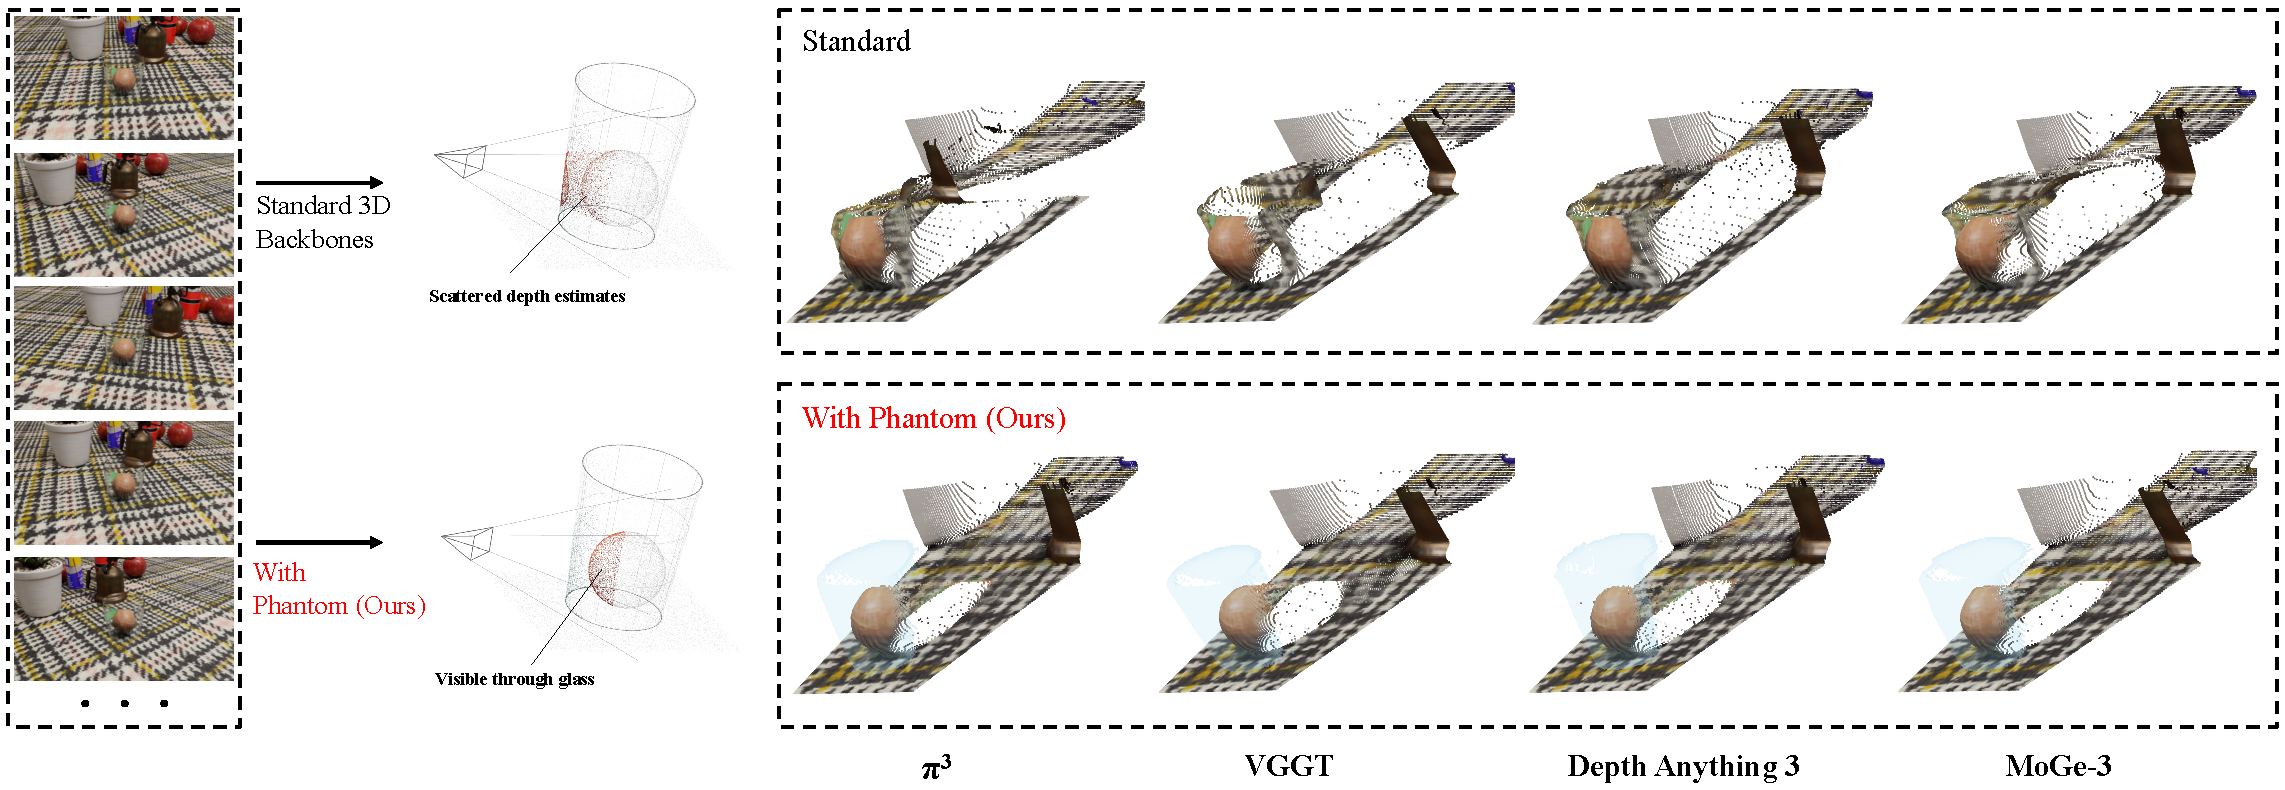
\includegraphics[width=\textwidth]{fig/teaser_slide5.pdf}
\captionsetup{hypcap=false}
\captionof{figure}{\textbf{Seeing through glass with Phantom.}
Input views and a conceptual illustration (left), followed by qualitative point-cloud comparisons using $\pi^3$, VGGT, Depth Anything 3, and MoGe-3 (right).
The top row shows the original backbones; the bottom row shows the corresponding results with Phantom, visualizing the recovered scene behind glass together with the transparent surface.}
\captionsetup{hypcap=true}
\label{fig:teaser}%
\end{strip}

\begin{abstract}
Feed-forward 3D reconstruction enables direct geometry prediction from single or sparse images, significantly reducing the dependency on per-scene iterative optimization and offering a new paradigm for efficient 3D perception and scene modeling. However, reconstructing transparent objects remains constrained by the inherent ambiguity of single-layer depth representations, where a single pixel often captures both the reflective surface of the glass and the occluded background scene. This ambiguity leads to two fundamental challenges: 1) depth estimation confusion between the transparent surface and the background, and 2) the inability to recover occluded background geometry when refraction occurs. To address these issues, we propose \textbf{Phantom}, a layered geometry reconstruction framework designed for frozen 3D geometry backbones. Phantom employs two complementary image front-ends to decouple the visual signals in the image domain: it independently extracts the interference-free background scene and the opaque surface appearance. We further introduce a geometry-aware loss based on frozen depth networks to suppress subtle artifacts that often induce erroneous surface predictions. Phantom demonstrates exceptional versatility and can be directly integrated with various state-of-the-art geometry backbones (e.g., VGGT, $\pi^3$, DA-V2 Metric, DA3, MoGe-2, and MoGe-3). Experimental results on the ClearGrasp dataset show that Phantom significantly reduces depth errors for transparent surfaces across all backbone models while effectively preserving the underlying background geometry. Finally, to facilitate the learning and evaluation of layered 3D geometry, we introduce, to our knowledge, the first multi-view synthetic dataset that pairs each transparent scene image with camera-aligned ground truth backgrounds, opaque surface references, and dual-layer depth annotations. Our code, pre-trained models, and dataset will be made publicly available.
\end{abstract}
    
\section{Introduction}
\label{sec:intro}

Feed-forward 3D reconstruction predicts geometry directly from one or a few images and avoids the per-scene optimization of classical pipelines~\cite{colmap,mvs}.
Models such as DUSt3R, VGGT and $\pi^3$~\cite{dust3r,vggt,pi3} have made this practical for opaque scenes, but the success does not carry over to transparent objects.
Facing a glass, they cannot tell its front surface from the background seen through it and predict a depth that mixes the two.

Transparent objects are difficult for two reasons.
Refraction and view-dependent reflections break the link between image texture and physical surfaces, which complicates depth estimation and cross-view matching~\cite{cleargrasp,lookingglass,neto}.
In addition, a pixel inside a transparent region observes two surfaces, the object and the scene behind it, while a depth map stores one value per pixel.
Better surface depth alone therefore cannot recover the background, and a layered representation is needed~\cite{ldi,photo3d}.

Existing methods recover a single layer.
ClearGrasp and TransCG complete the depth of the transparent surface from RGB and sensor depth~\cite{cleargrasp,transcg}, and GHOST renders the object opaque so that off-the-shelf geometry models perceive its surface without retraining~\cite{ghost}.
Image inpainting~\cite{partialconv,lama,mat} removes the object instead, but it replaces what is visible through the glass with plausible content.
Recovering both layers requires an image for each layer and a way to bring their two geometry predictions into one frame.

We propose \textbf{Phantom}, a layered reconstruction framework for frozen geometry backbones.
Given a transparent-object mask predicted by TransDINO~\cite{ghost}, two image front-ends translate the input into images that a backbone already handles well: a background front-end removes the transparent objects while keeping what is seen through them, and a surface front-end renders them opaque.
The backbone predicts geometry from each image without fine-tuning, and the two predictions are aligned on the pixels outside the mask and merged into a layered point cloud.
The same front-ends work with VGGT~\cite{vggt}, $\pi^3$~\cite{pi3}, Depth Anything V2 Metric~\cite{dav2}, Depth Anything 3~\cite{da3}, MoGe-2~\cite{moge2} and MoGe-3~\cite{moge3}.
On synthetic scenes they lower the error of both layers on all six backbones, and on real ClearGrasp images they lower the front-surface error more than GHOST.

Our contributions are:
\begin{itemize}
    \item Phantom, a layered reconstruction framework that recovers the transparent front surface and the scene behind it with two image front-ends and a frozen geometry backbone.
    \item One pair of front-ends that works with six frozen backbones without fine-tuning, improving both layers on synthetic data and the front surface on real images.
    \item To our knowledge, the first multi-view synthetic dataset with camera-aligned ground truth for both the background and the transparent surface, which we will release.
\end{itemize}

% Queue the two-column overview on page 2 so it appears at the top of page 3.
\begin{figure*}[t]
  \centering
  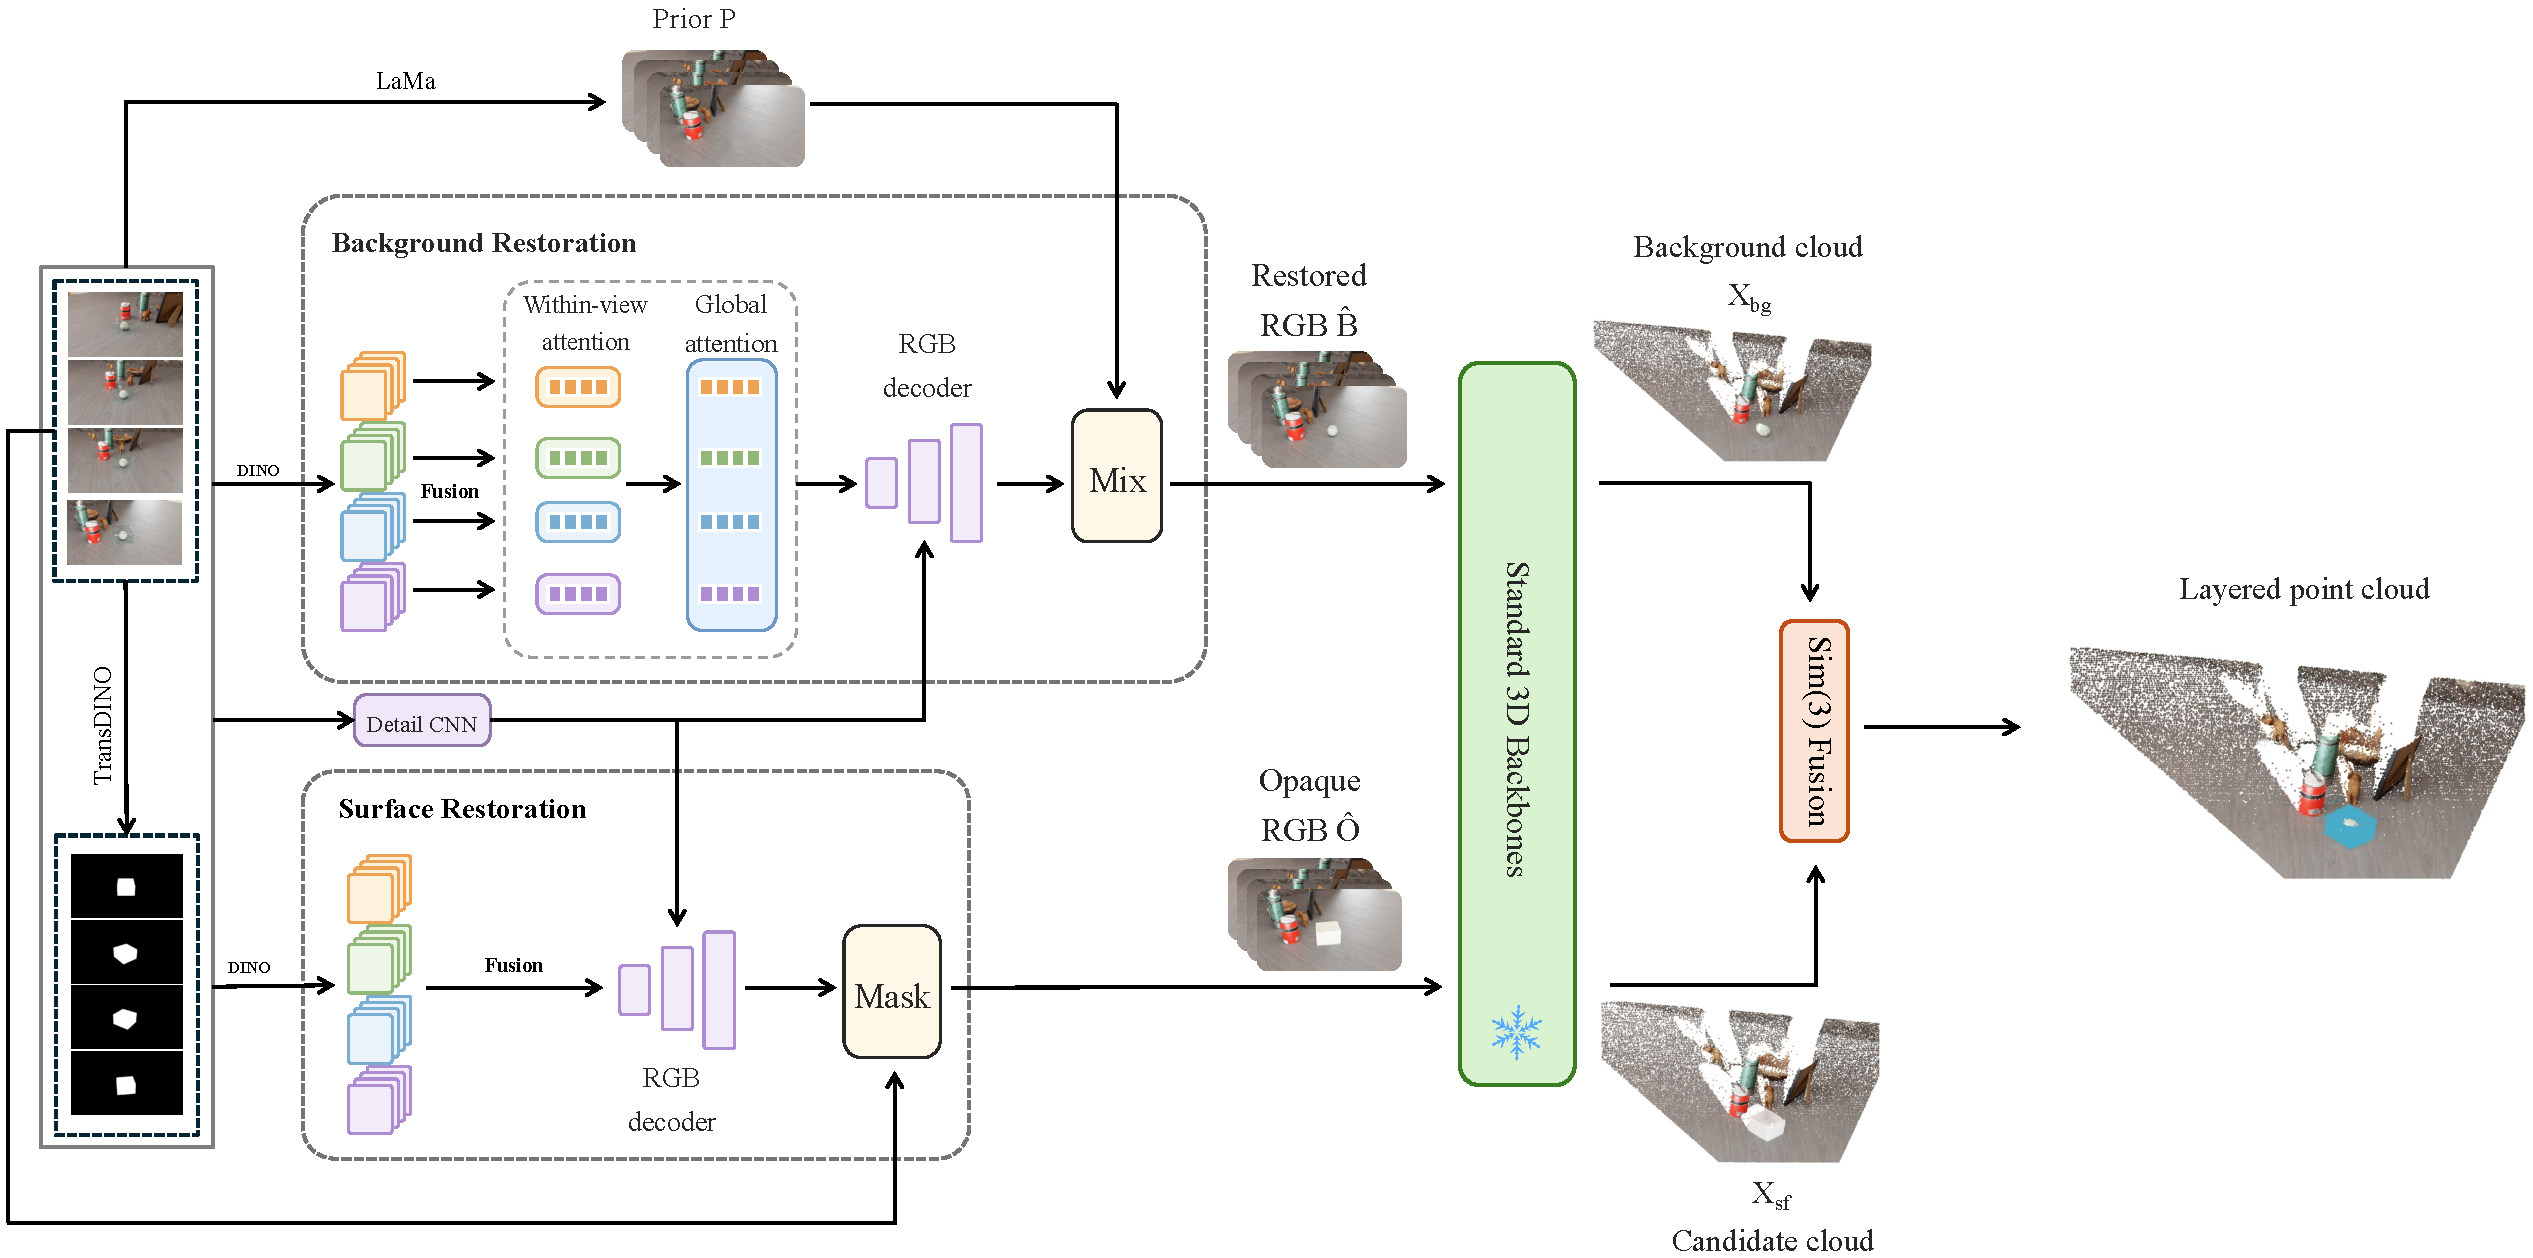
\includegraphics[width=\textwidth]{fig/method/output/architecture_slide3.pdf}
  \caption{\textbf{Overview of Phantom.}
  Given views $I$ and TransDINO masks $\hat M$~\cite{ghost}, the background front-end $\mathcal{F}_{bg}$ restores the scene behind the glass, $\hat B$, with attention across all views and a per-pixel mix with a LaMa prior $P$; the surface front-end $\mathcal{F}_{sf}$ renders the object opaque in each view, $\hat O$.
  A frozen geometry backbone $\mathcal{G}$ maps $\hat B$ and $\hat O$ to point clouds $X_{bg}$ and $X_{sf}$, which are aligned outside the mask and merged into a layered point cloud.}
  \label{fig:method}
\end{figure*}

\section{Related Work}
\label{sec:related}

\subsection{Feed-Forward 3D Reconstruction}
Classical structure-from-motion and multi-view stereo recover cameras and scene structure through matching, triangulation and optimization~\cite{colmap,mvs}, and MVSNet learns the cost-volume regularization~\cite{mvsnet}.
DUSt3R and MASt3R regress point maps from image pairs~\cite{dust3r,mast3r}, and VGGT and $\pi^3$ extend this to image collections~\cite{vggt,pi3}.
Monocular models trained at scale, from MiDaS and DPT~\cite{midas,dpt} to Depth Anything~\cite{depthanything,dav2,da3} and MoGe~\cite{moge,moge2,moge3}, often built on pretrained features such as DINOv2~\cite{dinov2}, give strong geometry priors for opaque scenes.
All of them predict one depth per pixel and do not separate a transparent front surface from the scene behind it.
Phantom keeps these models frozen and changes only their input.

\subsection{Transparent Scene Reconstruction}
Most work on transparent objects recovers the front surface.
ClearGrasp combines predicted normals and occlusion boundaries with depth optimization~\cite{cleargrasp}, while TransCG with DFNet~\cite{transcg}, local implicit functions~\cite{lidf} and temporally consistent prediction~\cite{consistentdepth} complete sensor depth.
Other work estimates keypoints and pose~\cite{keypose,clearpose}, or segments transparent regions from boundary cues~\cite{trans10k} or polarization~\cite{polarseg}.
Physically based methods model refraction to reconstruct object shape~\cite{lookingglass,neto}, and TOM-Net estimates refractive flow for environment matting~\cite{tomnet}.
Closest to ours, GHOST renders the object opaque so that off-the-shelf geometry models perceive its surface without retraining~\cite{ghost}.
Phantom uses the same image-domain idea for the surface, adds a second front-end that restores the background, and aligns the two predictions.

\subsection{Layered Representations and Inpainting}
Layered depth images store several depth and color samples per pixel~\cite{ldi}, multiplane images support view synthesis~\cite{stereomag,mpi}, and layered depth inpainting fills in content behind occluders for 3D photography~\cite{photo3d}.
NeRFReN separates transmitted and reflected radiance fields~\cite{nerfren}, and radiance-field and Gaussian representations~\cite{nerf,gs3d,pixelsplat,mvsplat} target novel-view rendering rather than per-layer geometry.
These works motivate keeping the hidden layer but do not model refraction.
Image inpainting~\cite{partialconv,contextual,gatedconv,lama,mat} can remove the object, but it fills the region with plausible content instead of keeping what is seen through the glass.
Phantom therefore uses LaMa only as a prior that its background front-end can override per pixel.

\section{Method}
\label{sec:method}

Phantom recovers two geometry layers from images of a scene with transparent objects: for every view, the visible front surface of each object and the scene seen through it.
Instead of training a new geometry network, we train two light image front-ends that translate the input into images a frozen, off-the-shelf geometry backbone already handles well, and then merge the backbone's two predictions (\cref{fig:method}).

\subsection{Problem Formulation}
\label{sec:formulation}

Given $N \ge 1$ views of the same scene, we denote the $i$-th view with known camera intrinsics $K_i$ as
\[
  I_i \in [0,1]^{H \times W \times 3}, \qquad i=1,\ldots,N.
\]
For each view, TransDINO~\cite{ghost} predicts the transparent-object mask
\[
  \hat M_i = \operatorname{TransDINO}(I_i) \in \{0,1\}^{H \times W}.
\]
Inside the mask, a pixel observes two surfaces at once: the front surface of the transparent object and, refracted and attenuated, the scene behind it.
A geometry backbone trained on opaque scenes predicts neither reliably and typically returns a mixture of the two.
We therefore assign each layer its own image:
\begin{equation}
  \begin{aligned}
  \{\hat B_i\}_{i=1}^{N} &= \mathcal{F}_{bg}\big(\{I_i, \hat M_i, P_i\}_{i=1}^{N}\big), \\
  \hat O_i &= \mathcal{F}_{sf}(I_i, \hat M_i),
  \end{aligned}
  \label{eq:frontends}
\end{equation}
where $\hat B_i$ is view $i$ with the transparent objects removed (objects behind or inside them are kept), $\hat O_i$ is the same view with every transparent object rendered as an opaque diffuse surface, and $P_i$ is a LaMa inpainting~\cite{lama} of $I_i$ inside $\hat M_i$.
$\mathcal{F}_{bg}$ receives all views of the scene and can exchange information between them; $\mathcal{F}_{sf}$ handles each view on its own.
Everything after the front-ends is done per view, so from here on we drop the view index.
A frozen geometry backbone $\mathcal{G}$ predicts a depth map for each image, which we back-project with $K$ (denoted $\Pi_K^{-1}$) into the background cloud $X_{bg}$ and the candidate surface cloud $X_{sf}$:
\begin{equation}
  X_{bg} = \Pi_K^{-1}\big(\mathcal{G}(\hat B)\big), \qquad X_{sf} = \Pi_K^{-1}\big(\mathcal{G}(\hat O)\big).
  \label{eq:backbone}
\end{equation}
$\mathcal{G}$ is any single-image or feed-forward geometry model; we use VGGT~\cite{vggt}, $\pi^3$~\cite{pi3}, Depth Anything V2 Metric~\cite{dav2}, Depth Anything 3~\cite{da3}, MoGe-2~\cite{moge2} and MoGe-3~\cite{moge3} without fine-tuning.
The front-ends are trained once and reused for every backbone.

\subsection{Front-End Architecture}
\label{sec:architecture}

$\mathcal{F}_{bg}$ and $\mathcal{F}_{sf}$ use the same encoders, decoder and output head (\cref{fig:method}) but are trained separately and keep separate weights.
Only $\mathcal{F}_{bg}$ has the prior input and the cross-view attention.
Both work at $294 \times 518$ and edit only the masked region.

% TODO(data swap): state the DINOv3 variant actually used. The code supports ViT-S/16 (layers 3/6/9/12)
% and ViT-L/16 (layers 6/12/18/24); the text below holds for both.
\paragraph{Encoders.}
A frozen DINOv3 ViT~\cite{dinov3} provides semantic context on a $21 \times 37$ token grid.
The mask enters through a zero-initialized patch convolution added to the tokens, so training starts from the pretrained features.
Tokens from four evenly spaced layers are projected, concatenated and fused by two $3{\times}3$ convolutions (\emph{Fusion} in \cref{fig:method}).
Because these features have only $1/16$ of the image resolution, a small trainable CNN computes detail features at $1/2$, $1/4$ and $1/8$ resolution from $I$, $\hat M$ and, for $\mathcal{F}_{bg}$, $P$.

% TODO(data swap): 4 attention pairs, 6 heads and 4 training views are the settings of the existing
% multi-view run (bg_mv4); confirm them for the final DINOv3 model.
\paragraph{Cross-view attention.}
In $\mathcal{F}_{bg}$, the fused features of the $N$ views pass through four pairs of attention blocks before decoding; each pair applies self-attention within each view and then across all views, following VGGT~\cite{vggt}.
Zero-initialized residual scales make the module start as the identity.
It uses no camera poses, depth or epipolar constraints; $\mathcal{F}_{sf}$ has no attention layers.

\paragraph{Decoder and output head.}
A convolutional decoder (\emph{RGB decoder} in \cref{fig:method}) upsamples the features in three stages, concatenating the detail features of matching resolution at each stage, and at full resolution concatenates the input image, the mask and (for $\mathcal{F}_{bg}$) the prior.
A single $3{\times}3$ convolution produces all outputs.
The main output is an RGB residual $r$ applied in logit space,
\begin{equation}
  C = \sigma\big(r + \operatorname{logit}(\operatorname{clip}(I, 0.02, 0.98))\big),
  \label{eq:residual}
\end{equation}
so that a zero residual reproduces the (clipped) input.
$\mathcal{F}_{bg}$ also outputs two fusion logits $(\ell_c, \ell_p)$ that select, per pixel, between its own prediction $C$ and the LaMa prior $P$ (\emph{Mix} in \cref{fig:method}).

\paragraph{Masked composition.}
Both front-ends paste their prediction into the input inside the mask (\emph{Mask} in \cref{fig:method}; for $\mathcal{F}_{bg}$ this step is part of \emph{Mix}).
To avoid seams at the mask boundary, we feather the mask, $\tilde M = \operatorname{AvgPool}_5(\operatorname{MaxPool}_5(\hat M))$, and compose
\begin{align}
  \hat B &= \tilde M \odot (w_c C_{bg} + w_p P) + (1 - \tilde M) \odot I, \label{eq:compose-bg} \\
  \hat O &= \tilde M \odot C_{sf} + (1 - \tilde M) \odot I, \label{eq:compose-sf}
\end{align}
where $(w_c, w_p) = \operatorname{softmax}(\ell_c, \ell_p)$ per pixel, and $C_{bg}$ and $C_{sf}$ are the outputs of \cref{eq:residual} for the two front-ends.

\subsection{Training Objective}
\label{sec:training}

Each front-end is trained on synthetic data (\cref{sec:data}) against its own target image $Y^*$: the rendered background $B^*$ for $\mathcal{F}_{bg}$ and the rendered opaque image $O^*$ for $\mathcal{F}_{sf}$.
Let $\hat Y$ be the front-end output, $M$ the ground-truth mask, $R$ the mask dilated by 3\,px, and $T \subseteq M$ the through region, where the background seen through the glass is another object rather than the support surface.
The loss is
\begin{equation}
  \begin{split}
  \mathcal{L} = {}&\mathcal{L}_{1} + \lambda_{p}\mathcal{L}_{\mathrm{LPIPS}} + \lambda_{o}\mathcal{L}_{\mathrm{out}} \\
  &+ \lambda_{f}\mathcal{L}_{\mathrm{flow}} + \lambda_{v}\mathcal{L}_{\mathrm{vis}} + \lambda_{g}\mathcal{L}_{\mathrm{geo}}.
  \end{split}
  \label{eq:loss}
\end{equation}

\paragraph{Image terms.}
$\mathcal{L}_{1}$ is the per-pixel L1 error weighted by $\omega = R \odot (1 + \lambda_t T)$ and normalized by $\sum \omega$.
For $\mathcal{F}_{bg}$ we set $\lambda_t = 2$, so through pixels, which carry the information that inpainting cannot provide, count three times; for $\mathcal{F}_{sf}$, $\lambda_t = 0$.
$\mathcal{L}_{\mathrm{LPIPS}}$ is the VGG LPIPS distance~\cite{lpips} between $Y^*$ and an image that equals $\hat Y$ inside $R$ and $Y^*$ elsewhere, divided by the area fraction of $R$.
$\mathcal{L}_{\mathrm{out}}$ is the mean L1 error outside $R$ and keeps the feathered band close to the input.

\paragraph{Auxiliary refraction terms.}
Both front-ends also predict a backward refraction flow, which maps each masked pixel to the background pixel seen through the glass, and a logit for whether that point is visible; neither is used to form the output image.
$\mathcal{L}_{\mathrm{flow}}$ is the L1 error of this flow where the ground truth is defined and visible, and $\mathcal{L}_{\mathrm{vis}}$ is the binary cross-entropy of the visibility logit inside $R$.

\paragraph{Geometry-aware term.}
An image can be close to $Y^*$ in color and still lead a backbone to a different depth.
We therefore pass both $\hat Y$ and $Y^*$ through a frozen depth network $D$ (Depth Anything V2 Metric, ViT-S~\cite{dav2}) and penalize the mean-centered log-depth difference inside $R$:
\begin{equation}
  \begin{split}
  \Delta &= \log D(\hat Y) - \log D(Y^*), \\
  \mathcal{L}_{\mathrm{geo}} & = \frac{1}{|R|}\sum_{x \in R} \Big|\Delta(x) - \bar\Delta_R\Big|,
  \end{split}
  \label{eq:geo}
\end{equation}
where $\bar\Delta_R$ is the mean of $\Delta$ over $R$.
Subtracting the mean makes the term invariant to a global depth scale, and because it compares two predictions of $D$, it needs no ground-truth depth.
$D$ is smaller than, and separate from, the backbones used at test time.

\paragraph{Settings.}
We use $\lambda_p = \lambda_o = 0.2$, $\lambda_f = 0.05$, $\lambda_v = 0.1$ and $\lambda_g = 0.5$ for both front-ends.
The input mask is the ground-truth mask with random morphological perturbations, so the front-ends learn to handle imperfect masks.
% TODO(data swap): batch size and views per scene of the final multi-view F_bg run.
Each front-end is trained for 40k iterations with AdamW~\cite{adamw}, and $\mathcal{F}_{bg}$ on groups of four views of the same scene.
Only the mask adapter, detail CNN, cross-view attention, decoder and head are trained.
Augmentations and optimizer settings are given in the supplement.

\begin{figure}[t]
  \centering
  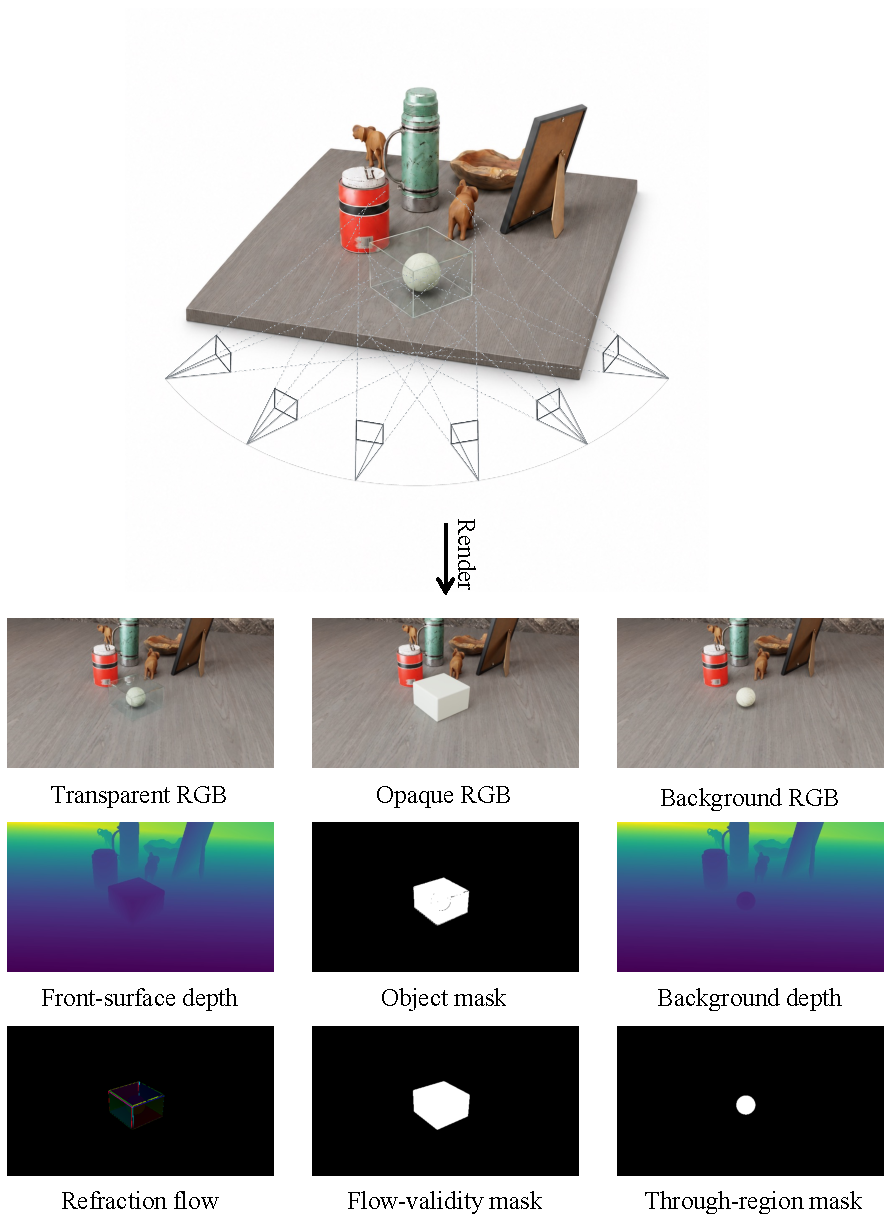
\includegraphics[width=\columnwidth]{fig/dataset/output/dataset_slide4.pdf}
  \caption{\textbf{Synthetic two-layer data.}
  Top: multi-view rendering setup.
  Bottom: per-view inputs and targets (RGB, opaque and background images, both depths, mask, refraction flow, flow validity and through region).}
  \label{fig:synthetic-data}
\end{figure}

\subsection{Layered Geometry Fusion}
\label{sec:fusion}

Because $\mathcal{G}$ runs on $\hat B$ and $\hat O$ separately, its two predictions are related by an unknown similarity transform, and backbones that predict only relative depth add a free scale.
We estimate this transform from the region where the two images agree.

\paragraph{Correspondences.}
Let $\Omega$ be the pixels outside $\hat M$ dilated by 7\,px at which both predictions are valid.
Outside the mask, $\hat B$ and $\hat O$ show the same scene, so for $x \in \Omega$ the points $X_{sf}(x)$ and $X_{bg}(x)$ should coincide.
These same-pixel pairs serve as correspondences and require no feature matching.
We randomly hold out 20\% of $\Omega$ for diagnostics and sample at most 8,000 of the remaining pixels for fitting.

\paragraph{Robust Sim(3).}
We seek $(s, \mathbf{R}, \mathbf{t})$ that minimize
\begin{equation}
  \sum_{x \in \Omega_{\mathrm{in}}} \big\| s\mathbf{R}\,X_{sf}(x) + \mathbf{t} - X_{bg}(x) \big\|^2 ,
  \label{eq:sim3}
\end{equation}
where $\Omega_{\mathrm{in}}$ is the set of inliers.
The predictions near depth discontinuities and in the feathered band can disagree strongly, so a plain least-squares fit over all of $\Omega$ is unreliable.
We run 250 RANSAC~\cite{ransac} iterations, each fitting a closed-form Umeyama~\cite{umeyama} solution to 6 random pairs and counting pairs with residual below $\tau = 0.025\,\mathrm{med}_{x}\|X_{bg}(x)\|$.
The hypothesis with the most inliers is refined by refitting on its inliers five times.

\paragraph{Layered point cloud.}
The final representation keeps every background point and adds the aligned surface points inside the mask:
\begin{equation}
  \mathcal{P} = \big\{X_{bg}(x)\big\}_{x} \;\cup\; \big\{s\mathbf{R}\,X_{sf}(x) + \mathbf{t} \;\big|\; \hat M(x) = 1\big\}.
  \label{eq:fusion}
\end{equation}
Each point carries a layer label: background outside the mask (0), background seen through the transparent object (1), and transparent front surface (2).
Inside the mask, the scene therefore has two depths per pixel, which a single prediction from $\mathcal{G}$ cannot represent.
Since $X_{bg}$ is the anchor, it fixes the scale and pose of the whole layered scene; it inherits any scale ambiguity of $\mathcal{G}$.

\subsection{Synthetic Two-Layer Data}
\label{sec:data}

Real images with ground truth for both the front surface and the scene behind it are not available, so we render training data with Blender Cycles (\cref{fig:synthetic-data}).
Each scene places transparent objects (cups, glasses, bottles, bowls, boxes, solid glass and thin films) on a textured table under indoor HDRI lighting, with scanned opaque props behind them and, in some containers, inside them, and is viewed by several cameras.
For every view we render the input $I$, the background target $B^*$ with all transparent objects hidden, the opaque target $O^*$ with every transparent material replaced by an opaque diffuse one, the masks $M$ and $T$, the depth of both layers, and the refraction flow.
Because all targets share the camera and lighting of $I$, the supervision isolates the effect of the transparent object.
We render three sets: \emph{Oblique} (4 oblique cameras per scene, 4--8 props), \emph{Clutter} (6--11 props, half of the scenes seen from nearly above as by a robot-arm camera, opaque labels and thicker glass) and \emph{Wide} (Clutter scenes seen by 6 cameras covering about 125\textdegree).
Rendering parameters are given in the supplement.

\section{Experiments}
\label{sec:experiments}

% Data sources: outputs/ablation_20261113/{tables,layered/v3w,robustness}
% and outputs/cleargrasp_ghost_20261116/summary.json.
% Split names: Oblique = synth_two_layer_v2, Clutter = v3, Wide = v3w.
% The current "Ours" and ablation values come from ab26_* runs with
% ResNet-50 single-view front-ends and ground-truth input masks in the standard evaluations.
% The "w/o DINOv3 features" rows currently report the ResNet-50 semantic-feature ablations.
% ClearGrasp's GHOST baseline is ghost_pred, which uses its own TransDINO masks.
% TODO: replace the provisional values with runs matching Section 3 and add the cross-view ablation.

\subsection{Setup}
\label{sec:exp-setup}

\paragraph{Data.}
We train on 7,776 views from scenes 60 and above of Oblique and Clutter (\cref{sec:data}), select checkpoints by masked PSNR on scenes 0--59 of Oblique, and test on scenes 0--59 of all three sets: Oblique (240 views), Clutter (240) and Wide (360).
Wide is used neither for training nor for checkpoint selection, so it is our main synthetic benchmark; full Oblique and Clutter tables are in the supplement.
For real images we use the 113 images of the ClearGrasp real-test split~\cite{cleargrasp}, which has ground truth for the front surface only and is never seen in training.
The input mask $\hat M$ is predicted by TransDINO~\cite{ghost} in all experiments, and one pair of front-ends serves all six backbones.
% TODO(data swap): confirm the number of views F_bg receives at test time (ClearGrasp images are single views).
$\mathcal{F}_{bg}$ receives all views of a synthetic test scene jointly; $\mathcal{F}_{sf}$ and the backbones run per view.

\paragraph{Baselines.}
\emph{Original} feeds the input $I$ to the backbone.
\emph{LaMa} feeds the inpainting $P$, which removes the glass together with what is seen through it (background layer only).
\emph{GHOST}~\cite{ghost} renders the object opaque and yields one layer, so we feed its output to the same backbones and compare on the surface layer.
\emph{Oracle} feeds the target image ($B^*$, $O^*$, or on ClearGrasp the photograph with the objects painted opaque) and bounds what an image front-end can achieve.
\Cref{fig:exp-qualitative} compares point clouds from Original, GHOST, and Phantom across four backbones.

\paragraph{Protocol and metrics.}
Each depth map is scaled by its median ratio to the ground truth over valid pixels outside the ground-truth mask $M$ dilated by 7\,px.
This uses ground-truth depth, so we evaluate relative geometry inside the mask, not metric scale.
Metrics are computed inside $M$ on pixels where all compared methods are valid: AbsRel (\%), RMSE, and $\delta_{1.05}$, the share of pixels with $\max(d/d^*, d^*/d) < 1.05$.
For layered results, the two predictions are first aligned as in \cref{sec:fusion} from predicted points only, and one ground-truth scale, computed on the background, is applied to both layers.
The aligned surface is z-buffer reprojected and can leave pixels empty, so we also report coverage and $\delta_{1.05}^{\mathrm{all}}$, which counts empty pixels as failures.
Layer-order error is the share of mask pixels where the surface lies behind the background.
An alignment fails when the median residual on the held-out correspondences exceeds 4\% of the median point distance or, for RANSAC, when fewer than 30\% of the pairs are inliers.

\paragraph{Seeds and statistics.}
The main front-ends are trained with three seeds; we report mean$\pm$std for VGGT, $\pi^3$ and DA-V2 and seed~0 elsewhere.
A difference is significant when the 95\% CI of a paired bootstrap over scenes excludes zero for every available seed.

\providecommand{\sd}[1]{{\scriptsize$\pm$#1}}
\newcommand{\tbgray}[1]{\textcolor{gray}{#1}}
\newcommand{\tbgood}[2]{\expheat{ExpGood!#1!ExpMid}{#2}}
\newcommand{\tbpoor}[2]{\expheat{ExpMid!#1!ExpPoor}{#2}}

\begin{table*}[t]
\centering
\footnotesize
\renewcommand{\arraystretch}{1.0}
\setlength{\tabcolsep}{2pt}
\begin{tabular*}{\textwidth}{@{}l@{\extracolsep{\fill}}ccccccccccc@{}}
\toprule
 & \multicolumn{4}{c}{\emph{Background: full mask}} & \multicolumn{4}{c}{\emph{Background: through region}} & \multicolumn{3}{c}{\emph{Front surface}} \\
\cmidrule(lr){2-5}\cmidrule(lr){6-9}\cmidrule(lr){10-12}
Backbone & Original & LaMa & \textbf{Ours} & \tbgray{Oracle} & Original & LaMa & \textbf{Ours} & \tbgray{Oracle} & Original & \textbf{Ours} & \tbgray{Oracle} \\
\midrule
VGGT~\cite{vggt} & \tbpoor{0}{13.55} & \tbgood{93}{\underline{1.96}} & \tbgood{100}{\textbf{1.51\sd{.06}}} & \tbgray{0.89} & \tbpoor{0}{7.72} & \tbpoor{41}{\underline{6.70}} & \tbgood{100}{\textbf{2.73\sd{.08}}} & \tbgray{1.62} & \tbpoor{0}{\underline{9.09}} & \tbgood{100}{\textbf{4.25\sd{.32}}} & \tbgray{2.55} \\
$\pi^3$~\cite{pi3} & \tbpoor{0}{12.95} & \tbgood{99}{\underline{1.95}} & \tbgood{100}{\textbf{1.91\sd{.05}}} & \tbgray{0.76} & \tbpoor{0}{9.60} & \tbpoor{70}{\underline{7.18}} & \tbgood{100}{\textbf{2.66\sd{.12}}} & \tbgray{1.55} & \tbpoor{0}{\underline{7.89}} & \tbgood{100}{\textbf{3.13\sd{.22}}} & \tbgray{1.87} \\
DA-V2~\cite{dav2} & \tbpoor{0}{22.45} & \tbgood{92}{\underline{2.52}} & \tbgood{100}{\textbf{1.70\sd{.01}}} & \tbgray{1.40} & \tbpoor{0}{11.92} & \tbgood{1}{\underline{7.81}} & \tbgood{100}{\textbf{3.81\sd{.02}}} & \tbgray{2.37} & \tbpoor{0}{\underline{24.20}} & \tbgood{100}{\textbf{4.37\sd{.13}}} & \tbgray{3.62} \\
DA3~\cite{da3} & \tbpoor{0}{11.16} & \tbgood{84}{\underline{2.01}} & \tbgood{100}{\textbf{1.24}} & \tbgray{0.89} & \tbpoor{8}{\underline{7.11}} & \tbpoor{0}{7.27} & \tbgood{100}{\textbf{3.08}} & \tbgray{2.26} & \tbpoor{0}{\underline{9.81}} & \tbgood{100}{\textbf{3.69}} & \tbgray{2.87} \\
MoGe-2~\cite{moge2} & \tbpoor{0}{12.01} & \tbgood{100}{\textbf{1.90}} & \tbgood{70}{\underline{3.41}} & \tbgray{0.92} & \tbpoor{0}{9.24} & \tbpoor{69}{\underline{7.34}} & \tbgood{100}{\textbf{3.75}} & \tbgray{2.13} & \tbpoor{0}{\underline{7.54}} & \tbgood{100}{\textbf{4.10}} & \tbgray{2.92} \\
MoGe-3~\cite{moge3} & \tbpoor{0}{12.19} & \tbgood{100}{\textbf{2.05}} & \tbgood{63}{\underline{3.95}} & \tbgray{1.02} & \tbpoor{0}{9.50} & \tbpoor{86}{\underline{7.23}} & \tbgood{100}{\textbf{4.22}} & \tbgray{2.16} & \tbpoor{0}{\underline{7.21}} & \tbgood{100}{\textbf{4.22}} & \tbgray{2.87} \\
\bottomrule
\end{tabular*}
\caption{\textbf{Layered depth on Wide} (AbsRel \%, $\downarrow$; 360 views never used in training). Through denotes background objects seen through glass. In all tables, green/red indicate better/worse results within each comparison group; bold/underlined mark best/second best. Gray Oracle references are excluded.}
\label{tab:exp-synthetic}
\end{table*}

\begin{figure*}[t]
\centering
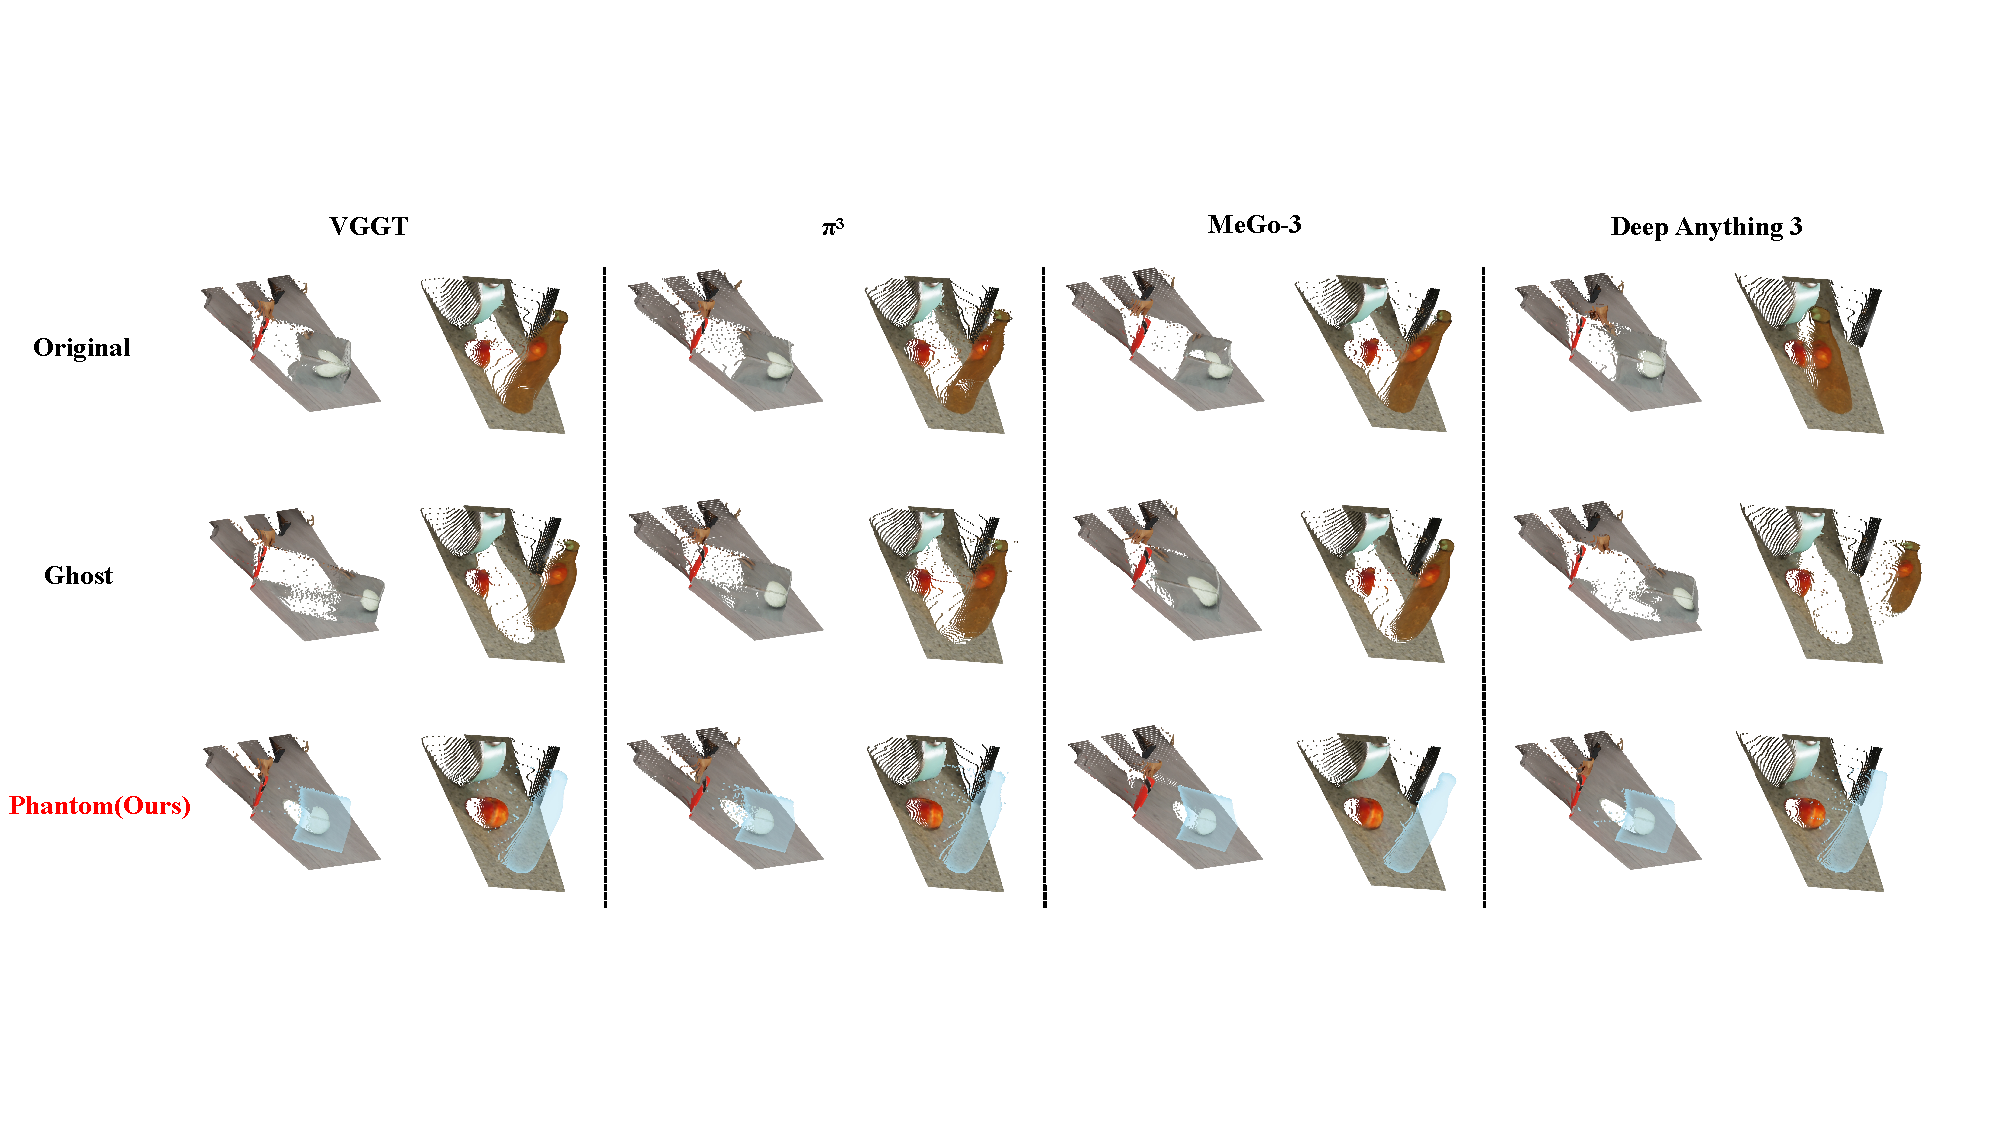
\includegraphics[pagebox=cropbox,width=\textwidth]{fig/qualitative_comparison.pdf}
\caption{\textbf{Qualitative point-cloud comparison.}
Each column group shows two example views for VGGT, $\pi^3$, MoGe-3, or Depth Anything 3.
From top to bottom, the rows show the original backbone, GHOST, and Phantom with the same backbone.}
\label{fig:exp-qualitative}
\end{figure*}

\subsection{Synthetic Layered Scenes}
\label{sec:exp-synthetic}

\Cref{tab:exp-synthetic} reports both layers on Wide.
With the original image, every backbone has 11--22\% AbsRel on the background and 7--24\% on the front surface, because it predicts one depth that mixes the two layers.
Phantom lowers the surface error on all six backbones, by 41\% (MoGe-3) to 82\% (DA-V2), and the background error to 1.2--4.0\%.

The through region shows what the background front-end adds over inpainting.
LaMa replaces the glass with a plausible table, which is correct for most mask pixels, so on the full mask it reaches 1.9--2.5\%.
Behind the glass, however, it hallucinates over the objects the camera actually sees, and its through-region error stays at 6.7--7.8\%, close to the Original.
Phantom keeps this content and reduces the through-region error to 2.7--4.2\% on every backbone.
On the full mask Phantom beats LaMa on four backbones but not on MoGe-2 and MoGe-3 (3.41 \vs 1.90 and 3.95 \vs 2.05).
We have not identified the cause; one possibility is that $\mathcal{L}_{\mathrm{geo}}$ uses a DA-V2 network whose preferences transfer poorly to MoGe.
Oblique and Clutter show the same pattern, including a slightly worse full-mask background than LaMa for $\pi^3$ (supplement).

\begin{table}[t]
\centering
\footnotesize
\renewcommand{\arraystretch}{1.0}
\setlength{\tabcolsep}{2pt}
\begin{tabular*}{\columnwidth}{@{}l@{\extracolsep{\fill}}ccccccc@{}}
\toprule
 & \multicolumn{4}{c}{AbsRel (\%, $\downarrow$)} & \multicolumn{3}{c}{RMSE (mm, $\downarrow$)} \\
\cmidrule(lr){2-5}\cmidrule(lr){6-8}
Backbone & Orig. & GHOST & \textbf{Ours} & \tbgray{Oracle} & Orig. & GHOST & \textbf{Ours} \\
\midrule
VGGT & \tbpoor{0}{7.84} & \tbgood{54}{\underline{4.00}} & \tbgood{100}{\textbf{2.86}} & \tbgray{2.35} & \tbpoor{0}{46.4} & \tbgood{46}{\underline{25.7}} & \tbgood{100}{\textbf{18.0}} \\
$\pi^3$ & \tbpoor{0}{6.71} & \tbgood{39}{\underline{4.14}} & \tbgood{100}{\textbf{3.02}} & \tbgray{1.98} & \tbpoor{0}{41.0} & \tbgood{37}{\underline{26.1}} & \tbgood{100}{\textbf{19.3}} \\
DA-V2 & \tbgood{56}{\underline{3.71}} & \tbpoor{0}{4.94} & \tbgood{100}{\textbf{3.36}} & \tbgray{2.81} & \tbgood{72}{\underline{23.4}} & \tbpoor{0}{30.9} & \tbgood{100}{\textbf{22.2}} \\
DA3 & \tbpoor{0}{4.79} & \tbpoor{1}{\underline{4.78}} & \tbgood{100}{\textbf{3.44}} & \tbgray{1.89} & \tbpoor{46}{\underline{29.0}} & \tbpoor{0}{31.1} & \tbgood{100}{\textbf{21.9}} \\
MoGe-2 & \tbpoor{0}{10.09} & \tbgood{35}{\underline{5.92}} & \tbgood{100}{\textbf{3.90}} & \tbgray{1.89} & \tbpoor{0}{57.1} & \tbgood{27}{\underline{35.9}} & \tbgood{100}{\textbf{23.8}} \\
MoGe-3 & \tbpoor{0}{9.80} & \tbgood{43}{\underline{5.20}} & \tbgood{100}{\textbf{3.38}} & \tbgray{1.62} & \tbpoor{0}{55.2} & \tbgood{38}{\underline{31.8}} & \tbgood{100}{\textbf{21.2}} \\
\midrule
Mean & \tbpoor{0}{7.16} & \tbgood{22}{\underline{4.83}} & \tbgood{100}{\textbf{3.33}} & \tbgray{2.09} & \tbpoor{0}{42.0} & \tbgood{13}{\underline{30.2}} & \tbgood{100}{\textbf{21.1}} \\
\bottomrule
\end{tabular*}
\caption{\textbf{Front-surface depth on ClearGrasp real-test} (113 images, inside the ground-truth mask). GHOST and Ours receive the same TransDINO masks. Ours is trained on synthetic data only; GHOST uses its released weights. Colors compare methods within each backbone and metric.}
\label{tab:exp-real}
\end{table}

\subsection{Real Transparent Objects}
\label{sec:exp-real}

\Cref{tab:exp-real} evaluates the front surface on ClearGrasp.
Phantom has the lowest error of the non-Oracle inputs on all six backbones and lowers the mean AbsRel from 7.16\% to 3.33\%, compared with 4.83\% for GHOST.
The gain is largest where the original prediction fails most (MoGe-2: 10.09 to 3.90\%); DA-V2, which already handles these images fairly well, improves from 3.71 to 3.36\%.
GHOST improves four backbones but is worse than Original on DA-V2 (4.94\%) and on par with it on DA3 (4.78\%).
Both methods inherit the errors of TransDINO, whose masks reach a mean IoU of 0.74 on these images (median 0.88; 23 of 113 below 0.5).
The remaining gap to the Oracle, 1.2 points on average, is the room left for a better surface front-end.

\begin{table}[t]
\centering
\footnotesize
\renewcommand{\arraystretch}{1.0}
\setlength{\tabcolsep}{3pt}
\begin{tabular*}{\columnwidth}{@{}l@{\extracolsep{\fill}}ccccc@{}}
\toprule
 & \multicolumn{2}{c}{AbsRel (\%) $\downarrow$} & \multicolumn{2}{c}{Order (\%) $\downarrow$} & $\delta^{\mathrm{all}}_{1.05}\uparrow$ \\
\cmidrule(lr){2-3}\cmidrule(lr){4-5}
Front-ends & Backgr. & Surface & VGGT & 6-mean &  \\
\midrule
None (Original) & \expheat{ExpMid!0!ExpPoor}{\underline{13.55}} & \expheat{ExpMid!0!ExpPoor}{9.09} & \textcolor{gray}{0.00$^\ast$} & \textcolor{gray}{0.00$^\ast$} & \expheat{ExpMid!13!ExpPoor}{52.7} \\
$\mathcal{F}_{bg}$ only & \expheat{ExpGood!100!ExpMid}{\textbf{1.55}} & \expheat{ExpMid!2!ExpPoor}{9.05} & \expheat{ExpGood!84!ExpMid}{\underline{2.41}} & \expheat{ExpGood!22!ExpMid}{\underline{7.84}} & \expheat{ExpMid!0!ExpPoor}{51.1} \\
$\mathcal{F}_{sf}$ only & \expheat{ExpMid!0!ExpPoor}{\underline{13.55}} & \expheat{ExpGood!99!ExpMid}{\underline{4.62}} & \expheat{ExpMid!0!ExpPoor}{23.34} & \expheat{ExpMid!0!ExpPoor}{17.89} & \expheat{ExpGood!100!ExpMid}{\textbf{76.7}} \\
\textbf{Both (Ours)} & \expheat{ExpGood!100!ExpMid}{\textbf{1.55}} & \expheat{ExpGood!100!ExpMid}{\textbf{4.60}} & \expheat{ExpGood!100!ExpMid}{\textbf{0.60}} & \expheat{ExpGood!100!ExpMid}{\textbf{1.38}} & \expheat{ExpGood!96!ExpMid}{\underline{76.2}} \\
\bottomrule
\end{tabular*}
\caption{\textbf{Branch combination} on Wide (VGGT, seed~0). A disabled branch uses the original image. Order denotes layer-order error (VGGT and six-backbone mean). $^\ast$Trivial zeros from identical predictions are excluded from ranking and coloring.}
\label{tab:exp-branches}
\end{table}

\subsection{Ablation Studies}
\label{sec:exp-analysis}

\paragraph{Both front-ends are needed.}
\Cref{tab:exp-branches} enables the front-ends one at a time.
Each front-end improves only its own layer.
With the surface front-end alone, the background is still the mixed original prediction, which lies in front of the restored surface at 23\% of the mask pixels for VGGT.
With both front-ends the layer-order error drops to 0.60\% for VGGT and to 1.38\% on average over the six backbones.
Adding the background front-end leaves the surface accuracy nearly unchanged (AbsRel 4.62 \vs 4.60, $\delta^{\mathrm{all}}_{1.05}$ 76.7 \vs 76.2), so the order improvement does not come at the cost of the surface.

\paragraph{Alignment.}
Averaged over the six backbones on Wide, fusing the two predictions without alignment fails in 44\% of the views (up to 86\% for MoGe-3) and gives 9.45\% surface AbsRel, because independent predictions differ in scale.
A single scale already removes most of the discrepancy (4.07\%, 0.05\% failures), and a least-squares Sim(3) fails in up to 5\% of the views of a backbone.
RANSAC Sim(3) has no failures and gives 4.16\% AbsRel; we use it by default, and scale-only alignment is a simpler alternative of similar accuracy (supplement).

\begin{table}[t]
\centering
\footnotesize
\renewcommand{\arraystretch}{1.0}
\setlength{\tabcolsep}{3pt}
\begin{tabular*}{\columnwidth}{@{}c@{\hspace{4pt}}l@{\extracolsep{\fill}}cccc@{}}
\toprule
& Variant & VGGT $\downarrow$ & $\pi^3\downarrow$ & DA-V2 $\downarrow$ & PSNR $\uparrow$ \\
\midrule
\multirow{9}{*}{\rotatebox{90}{$\mathcal{F}_{bg}$}}
 & w/o LaMa prior & \expheat{ExpMid!0!ExpPoor}{2.77\sd{.13}$^\dagger$} & \expheat{ExpMid!0!ExpPoor}{3.69\sd{.57}$^\dagger$} & \expheat{ExpGood!30!ExpMid}{1.78\sd{.01}} & \expheat{ExpMid!96!ExpPoor}{24.08\sd{.04}} \\
 & Prior as input only & \expheat{ExpGood!22!ExpMid}{2.00$^\dagger$} & \expheat{ExpGood!3!ExpMid}{2.69$^\dagger$} & \expheat{ExpGood!100!ExpMid}{\textbf{1.70}} & \expheat{ExpGood!73!ExpMid}{24.46} \\
 & Fixed 0.5/0.5 fusion & \expheat{ExpGood!48!ExpMid}{1.84$^\dagger$} & \expheat{ExpGood!9!ExpMid}{2.63$^\dagger$} & \expheat{ExpGood!48!ExpMid}{1.76$^\dagger$} & \expheat{ExpMid!96!ExpPoor}{24.08$^\dagger$} \\
 & w/o LPIPS & \expheat{ExpMid!65!ExpPoor}{2.36$^\dagger$} & \expheat{ExpMid!88!ExpPoor}{2.84$^\dagger$} & \expheat{ExpMid!0!ExpPoor}{1.93$^\dagger$} & \expheat{ExpGood!45!ExpMid}{24.32$^\dagger$} \\
 & w/o detail CNN & \expheat{ExpGood!86!ExpMid}{1.60\sd{.07}} & \expheat{ExpGood!60!ExpMid}{2.14\sd{.07}} & \expheat{ExpGood!74!ExpMid}{1.73\sd{.01}} & \expheat{ExpMid!51!ExpPoor}{23.86\sd{.06}$^\dagger$} \\
 & w/o DINOv3 & \expheat{ExpGood!78!ExpMid}{1.65} & \expheat{ExpGood!58!ExpMid}{2.16} & \expheat{ExpMid!43!ExpPoor}{1.88$^\dagger$} & \expheat{ExpMid!0!ExpPoor}{23.61$^\dagger$} \\
 & w/o $\mathcal{L}_{\mathrm{geo}}$ & \expheat{ExpGood!92!ExpMid}{1.56\sd{.01}} & \expheat{ExpGood!75!ExpMid}{1.99\sd{.02}} & \expheat{ExpGood!91!ExpMid}{\underline{1.71\sd{.03}}} & \expheat{ExpGood!100!ExpMid}{\textbf{24.59\sd{.04}}} \\
 & w/o $T$ weighting & \expheat{ExpGood!98!ExpMid}{\underline{1.52\sd{.04}}} & \expheat{ExpGood!100!ExpMid}{\textbf{1.75\sd{.11}}} & \expheat{ExpGood!100!ExpMid}{\textbf{1.70\sd{.02}}} & \expheat{ExpGood!86!ExpMid}{\underline{24.52\sd{.02}}} \\
 & \textbf{Full (Ours)} & \expheat{ExpGood!100!ExpMid}{\textbf{1.51\sd{.06}}} & \expheat{ExpGood!84!ExpMid}{\underline{1.91\sd{.05}}} & \expheat{ExpGood!100!ExpMid}{\textbf{1.70\sd{.01}}} & \expheat{ExpGood!73!ExpMid}{24.46\sd{.09}} \\
\midrule
\multirow{5}{*}{\rotatebox{90}{$\mathcal{F}_{sf}$}}
 & w/o $\mathcal{L}_{\mathrm{geo}}$ & \expheat{ExpMid!80!ExpPoor}{4.67\sd{.13}} & \expheat{ExpGood!42!ExpMid}{\underline{3.22\sd{.25}}} & \expheat{ExpGood!83!ExpMid}{4.60\sd{.31}} & \expheat{ExpGood!1!ExpMid}{19.03\sd{.10}} \\
 & w/o detail CNN & \expheat{ExpGood!9!ExpMid}{4.57\sd{.16}} & \expheat{ExpMid!0!ExpPoor}{3.44\sd{.31}} & \expheat{ExpGood!91!ExpMid}{\underline{4.49\sd{.11}}} & \expheat{ExpGood!100!ExpMid}{\textbf{19.53\sd{.37}}} \\
 & w/o DINOv3 & \expheat{ExpMid!0!ExpPoor}{4.95} & \expheat{ExpMid!0!ExpPoor}{3.44} & \expheat{ExpGood!57!ExpMid}{4.94} & \expheat{ExpMid!59!ExpPoor}{18.82} \\
 & w/o LPIPS & \expheat{ExpGood!63!ExpMid}{\underline{4.38}} & \expheat{ExpMid!77!ExpPoor}{3.32} & \expheat{ExpMid!0!ExpPoor}{7.03$^\dagger$} & \expheat{ExpMid!0!ExpPoor}{18.52$^\dagger$} \\
 & \textbf{Full (Ours)} & \expheat{ExpGood!100!ExpMid}{\textbf{4.25\sd{.32}}} & \expheat{ExpGood!100!ExpMid}{\textbf{3.13\sd{.22}}} & \expheat{ExpGood!100!ExpMid}{\textbf{4.37\sd{.13}}} & \expheat{ExpGood!17!ExpMid}{\underline{19.11\sd{.12}}} \\
\bottomrule
\end{tabular*}
\caption{\textbf{Component ablation} on Wide (AbsRel \%, and masked PSNR in dB). $^\dagger$: the paired scene-bootstrap 95\% CI of the difference to the full model excludes zero for every seed. Std uses three seeds; other rows use seed~0. Colors compare variants within each front-end and metric.}
\label{tab:exp-ablation}
\end{table}

\paragraph{Components.}
\Cref{tab:exp-ablation} removes one component at a time.
For the background, the LaMa prior and the learned fusion matter most.
Without the prior, VGGT's error rises from 1.51 to 2.77\%; giving the prior to the network only as an input (2.00\%) or mixing it with fixed weights (1.84\%) recovers part of the gap.
Removing LPIPS hurts every backbone.
The detail CNN and the DINOv3 features mainly improve the image (PSNR $-0.60$ and $-0.85$\,dB without them), with smaller changes in depth.
For the surface, every removal increases the mean error, but most differences are not significant in all seeds.
$\mathcal{L}_{\mathrm{geo}}$ reduces the VGGT surface error from 4.67 to 4.25\% on average, with a significant difference in two of three seeds, and has no measurable effect on the background.
Two non-default settings are better on Wide (geometry weight 1.0 for the background, no auxiliary terms for the surface); we fixed the defaults before the ablation and report these variants in the supplement.

\paragraph{Mask errors.}
Because Phantom edits only the masked region, a mask that misses part of the object leaves that part unchanged.
We perturb the input mask, recompute the LaMa prior, and keep the evaluation mask fixed (seed~0, VGGT / $\pi^3$ / DA-V2).
Dilating the mask by 3 or 7\,px does not hurt (background 1.1--2.0\%, surface 2.9--4.8\%, close to the unperturbed values).
A (3, 3)\,px shift raises the background error to 7.2--10.3\%, and a 3\,px erosion to 13.1--20.3\%, the level of the original image, with the VGGT surface error rising to 9.03\%.
Over-segmentation is therefore much safer than under-segmentation, and the mask predictor should be biased towards larger masks.

\subsection{Limitations}
\label{sec:exp-limitations}

Phantom depends on the mask: pixels it misses are not edited (\cref{sec:exp-analysis}).
There is no real benchmark with ground truth for both layers, so the hidden background is evaluated on synthetic data only, real images test only the front surface, and all depths are evaluated up to a ground-truth scale.
Only the background front-end uses several views, and its attention has no camera geometry; the backbone, the alignment and the fusion run per view, so the layered clouds of different views are not merged into one scene.
On MoGe-2 and MoGe-3 the restored background still trails LaMa, so the front-ends do not yet transfer equally well to every backbone.

\section{Conclusion}
\label{sec:conclusion}

We presented Phantom, which recovers the front surface of transparent objects and the scene behind them with a frozen geometry backbone.
Two image front-ends, one restoring the background and one rendering the object opaque, are trained once on synthetic data and used with six backbones without fine-tuning; the two predictions are aligned outside the mask and merged into a layered point cloud.
On synthetic scenes both layers improve on all six backbones, and on real ClearGrasp images the front-surface error is lower than with GHOST.
Phantom depends on the TransDINO mask and degrades when the mask misses part of the object.
The hidden background is evaluated on synthetic data only, so a real benchmark with ground truth for both layers is an important next step.
We will release the code, the trained front-ends and the synthetic dataset.

% Author-kit instructions are retained as source files, outside the paper body.
% \input{sec/2_formatting}
% \input{sec/3_finalcopy}
{
    \small
    \bibliographystyle{ieeenat_fullname}
    \bibliography{main}
}

% WARNING: do not forget to delete the supplementary pages from your submission 
% \input{sec/X_suppl}

\end{document}
